\documentclass{beamer}

\usepackage[latin1]{inputenc}
\usepackage{amsmath}
\usepackage{amssymb}

\usecolortheme[RGB={239,165,80}]{structure}
\useoutertheme{infolines}
\usetheme[height=10mm]{Rochester}
\setbeamertemplate{items}[circle]
\setbeamertemplate{blocks}[rounded][shadow=true]
\setbeamertemplate{navigation symbols}{}

\title[Degrees of belief]
      {An introduction to Bayesian probabilities and their application}

\author{Kieran Gorman}
%\institute{Xero}
%\date{2015}

\begin{document}

\begin{frame}
  \titlepage
\end{frame}


\begin{frame}{Probability}

  \begin{itemize}
    \setlength\itemsep{1em}
    \item How 'likely' is the occurrence of a certain event?
    \item Traditionally 'frequentist'.
    \item The limit given relative observed frequency.
    \item That is, having observed $P(x) \approx \frac{n_x}{n_t}$ we
      might deduce that $P(x) = \lim_{x\to\infty} \frac{n_x}{n_t}$
    \item In the frequentist model, a hypothesis is a well defined
      proposition (i.e. certainly true or certainly false).
  \end{itemize}

\end{frame}

\begin{frame}{Probability cont.}

  \begin{center}
    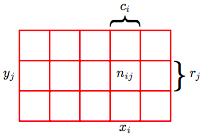
\includegraphics[scale=0.5]{pgrid}
  \end{center}

  \begin{itemize}
    \item Joint: $P(X = x_i, Y = y_j) = \frac{n_{ij}}{N}$
    \item Sum rule: $P(X = x_i) = \sum_{j=1}^{L}P(X = x_i, Y = y_j)$
    \item Conditional: $P(Y = y_j | X = x_i) = \frac{n_{ij}}{c_i}$ \\
      $P(X = x_i, Y = y_j) = \frac{n_{ij}}{N} = \frac{n_{ij}}{c_i}
      \cdot \frac{c_i}{N}$
    \item Product rule: $P(X = x_i, Y = y_j) = P(Y = y_j | X = x_i) \cdot
      P(X = x_i)$
  \end{itemize}

  \begin{center}
    {\tiny
      This also holds for continuous variables, as probability
      densities, just replace $\sum$ with $\int$
    }
  \end{center}

\end{frame}

\begin{frame}{Bayes Theorem}

  It's just an application of the sum and product rules.


  \begin{align}
    P(X, Y) &= P(Y, X) \nonumber \\
    P(Y|X) \cdot P(X) &= P(X|Y) \cdot P(Y) \nonumber \\
    P(Y|X) &= \frac{P(X|Y) \cdot P(Y)}{P(X)} \nonumber
  \end{align}

  We're not quite at actual Bayesian probabilities, but we can
  immediately begin to apply Bayes theorem in a classification problem.

\end{frame}

\begin{frame}{Na\"ive Bayes Classifier}

  Apply Bayes theorem, along with a strong independence assumption
  (this is what makes it 'na\"ive').

  \begin{align}
    p(C_k, x_1, \ldots, x_n) &= p(C_k)p(x_1, \ldots, x_n | C_k)
    \nonumber \\
    &= p(C_k)p(x_1|C_k)p(x_2, \ldots, x_n | C_k, x_1) \nonumber \\
    &= p(C_k)p(x_1|C_k)p(x_2|C_k, x_1)p(x_3,\ldots,c_n|C_k,x_1,x_2)
    \nonumber \\
    &= p(C_k)p(x_1|C_k)p(x_2|C_k,x_1)\ldots p(x_n|C_k,x_1,\ldots,
    x_{n-1}) \nonumber
  \end{align}

  Now assume all of the values in the input vector are independent of
  one another, meaning $P(A|B, C) = P(A|B) \cdot P(A|C)$. In our case
  it means that $p(x_i | C_k, x_j, x_k) = p(x_i | C_k)$.

\end{frame}

\begin{frame}{Na\"ive Bayes Classifier cont.}
  So, applying Bayes theorem we get

  \begin{align}
  P(C_k|x_1, \ldots, x_n) &\propto p(C_k) p(x_1,\ldots,x_n | C_k)
  \nonumber \\
  &\propto p(C_k) p(x_1 | C_k) p(x_2 | C_k) \ldots p(x_n | C_k)
  \nonumber \\
  &\propto p(C_k)\prod_{i=1}^{n}P(x_i | C_k) \nonumber
  \end{align}

  That is, the probability of labelling an input instance with a
  certain class is simply the probability of that class, multiplied by
  the likelihood that instance appearing in that class based on what
  we've seen already.


  {\tiny
    This assumption is clearly false in almost all interesting
    cases, however in general corpus is king. See ``Unreasonable
    effectiveness of data'', from Norvig.
  }

\end{frame}

\begin{frame}{Contrived demonstration}

  Demo.

\end{frame}

\begin{frame}{A Bayesian approach}

  We can interpret Bayes theorem as:

  \begin{align}
    p(A|B) &= \frac{p(B|A) \cdot p(A)}{p(B)} \nonumber \\
    &\propto p(B|A) \cdot p(A) \nonumber \\
    posterior &\propto likelihood \cdot prior \nonumber
  \end{align}

  We can see that by counting frequencies, we are fixing our
  probability estimator to one that maximises likelihood for computing
  $p(x)$. \\

  The Bayesian approach is to permit an uncertainty so our likelihood
  is not beholden to the evidence alone.

\end{frame}

\begin{frame}{A Bayesian approach cont.}

  \begin{itemize}
    \item Consider for example events we have a degree of belief in
      occurring, but we can't readily measure (say, the state of the
      polar ice caps at the turn of the next century).
    \item Frequencies require repeatability!
    \item Bayesian probabilities are sometimes called ``a logical
      approach to probabilities'' and can be derived from Cox's axioms
      (i.e. ``degrees of belief'') for example.
  \end{itemize}

\end{frame}

\begin{frame}

  \begin{itemize}
    \item In Frequentism we have a fixed input, and hypothesise about
      possible underlying datasets from which it might derive.
    \item In Bayesianism, we only have the observed data, and the
      uncertainty is in a probability distribution over the inputs.
    \item Using a maximum likelihood function over fixed inputs
      without catering for uncertainty in the hypothesis can lead to
      extreme conclusions.
  \end{itemize}

\end{frame}

\begin{frame}{Demo}
  A slightly more involved demo.
\end{frame}

\begin{frame}{Onwards}

  \begin{itemize}
    \item What if we want to model dependencies?
    \item Need more involved models!

    \item Bayesian networks: probabilistic graphical models that
      allow for belief propagation. (Look up Judea Pearl.)

    \item Can't generally be computed in a closed form.
  \end{itemize}

\end{frame}

\begin{frame}{Iterative models}
  \begin{itemize}
    \item Because we were using Gaussians as the underlying
      distribution of the na\"{i}ve classifier, we could compute the
      max-likelihood parameter set in a closed form.
    \item More complex models require a more explicit
      parameterisation.
    \item One example: neural networks.
  \end{itemize}
\end{frame}

\begin{frame}{Neural networks from 30,000ft}
  \begin{itemize}
    \item Given an input vector, produce an output vector.
    \item Compare output vector to target with some notion of
      ``fitness''
    \item Update weightings to increase fitness. Iterate.
  \end{itemize}
\end{frame}

\begin{frame}{Neural networks from 29,999ft}
  \begin{itemize}
    \item How to update?
    \item Back-propagation algorithm.
  \end{itemize}

  \begin{center}
    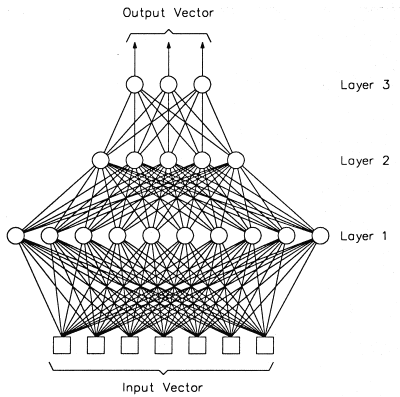
\includegraphics[scale=0.4]{multi}
  \end{center}
\end{frame}

\begin{frame}{Gradient descent search}
  \begin{itemize}
    \item In general: gradient descent search.
    \item Exploring a solution space.
    \item Can be parallelised and made more robust to local optima
      (particle swarm optimisation).
    \item In the context of probabilities basically just trying to
      integrate over parameter sets to find max-likelihood.
  \end{itemize}
\end{frame}

\begin{frame}{Intuitions}
  \begin{itemize}
    \item Overall: Bayesian probabilities provide a framework for
      working with uncertainty.
    \item In particular, having uncertain hypotheses maps conceptually
      well with automated pattern recognition.
    \item Lots of sampling and search techniques are basically just
      trying to avoid doing integrals.
  \end{itemize}
\end{frame}

\begin{frame}{Exeunt}
  \begin{itemize}
    \item Corpus is king.
    \item Uncertainty + priors implies parameterisation.
    \item Large amounts of ML is choosing good priors and heuristics
      for assumed latent distributions.
    \item Doesn't actually require a lot of math.
    \item It is lots of fun!
    \item Can we start being more data-directed at Xero? No more hard
      coded defaults or rules!
  \end{itemize}
\end{frame}

\begin{frame}{Thanks}
  Thanks!

  \begin{itemize}
    \item References:
    \begin{itemize}
      \item Bishop --- Pattern Recognition and Machine Learning
      \item Norvig --- Artificial Intelligence: A Modern Approach
      \item Data sets: UCI Machine Learning Repository
    \end{itemize}
  \end{itemize}
\end{frame}

\end{document}
